Si inverte la matrice precedentemente ottenuta:
$$
\begin{bmatrix}
Q_1\\
Q_2
\end{bmatrix} = \frac{4\pi \varepsilon_0}{\frac{1}{R_1R_2}-\frac{1}{d^2}} \begin{bmatrix}
\frac{1}{R_2} & -\frac{1}{d}\\
-\frac{1}{d} & \frac{1}{R_1}
\end{bmatrix}\begin{bmatrix}
V_1 \\
V_2
\end{bmatrix}
$$
Si ottengono quindi le capacità parziali:
\begin{align*}
&C_{11} = \frac{4\pi\varepsilon_0}{\frac{1}{R_1R_2}-\frac{1}{d^2}}\frac{1}{R_2} & C_{12} = 
\frac{4\pi\varepsilon_0}{\frac{1}{R_1R_2}-\frac{1}{d^2}}\left(-\frac{1}{d}\right)\\
&C_{22} = \frac{4\pi\varepsilon_0}{\frac{1}{R_1R_2}-\frac{1}{d^2}}\frac{1}{R_1} & C_{21} = 
\frac{4\pi\varepsilon_0}{\frac{1}{R_1R_2}-\frac{1}{d^2}}\left(-\frac{1}{d}\right)
\end{align*}
\begin{align*}
&C_{11}^* = C_{11} + C_{12} = \frac{4\pi\varepsilon_0}{\frac{1}{R_1R_2}-\frac{1}{d^2}}
\left(\frac{1}{R_2} - \frac{1}{d}\right)\\
&C_{22}^* = \frac{4\pi\varepsilon_0}{\frac{1}{R_1R_2}-\frac{1}{d^2}}
\left(-\frac{1}{d} + \frac{1}{R_1}\right)\\
&C_{12}^* = -\frac{4 \pi \varepsilon_0}{\frac{1}{R_1R_2}-\frac{1}{d^2}}\left(-\frac{1}{d}\right) =
\frac{4 \pi \varepsilon_0}{\left(\frac{1}{R_1R_2} - \frac{1}{d^2}\right)}\cdot\frac{1}{d} = \frac{4\pi\varepsilon_0 R_1R_2d}{d^2-R_1R_2}
\end{align*}

Se supponiamo che ci sia un fenomeno di induzione completa: 
$$
Q_2 = -Q_1 \Rightarrow C = C_{12}^* +
\left(\frac{1}{C_{11}^*} + \frac{1}{C_{22}^*}\right)^{-1}
$$
$$
C = \frac{Q_1}{V_1-V_2} = \frac{1}{\frac{1}{4\pi\varepsilon_0}}\frac{Q_1}{\frac{Q_1}{R_1} -
\frac{Q_1}{d}-\left(\frac{Q_1}{d}-\frac{Q_1}{R_2}\right)} =
\frac{4\pi\varepsilon_0}{\frac{1}{R_1} + \frac{1}{R_2} - \frac{2}{d}}
$$
Eseguendo il limite per $d\to \infty$ si vede che l'espressione precedente è coerente con quella 
ricavata nell'ipotesi in cui le cariche siano poste a grande distanza.


\subparagraph{Capacità per unità di lunghezza di una linea bifilare}

I due conduttori possono essere rappresentati mediante due sezioni cilindriche,
le cariche associate $Q_1$ e $Q_2$ si accumuleranno per unità di lunghezza e 
saranno quindi misurate in \si{\coulomb\per\meter}.
Applicando il PSE
\begin{figure}[h!]
\centering
 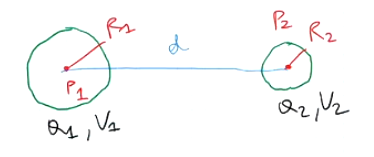
\includegraphics[width=0.5\linewidth]{conduttori_bifilari}
\caption{Sezione conduttori bifilari}
\end{figure} 

\begin{align*}
V_1' &= -\frac{\sigma_1 R_1}{\varepsilon_0} \ln R_1 & V_2' &= -\frac{\sigma_1 R_1}{\varepsilon_0} \ln d\\
V_1'' &= -\frac{\sigma_2 R_2}{\varepsilon_0} \ln d & V_2'' &= -\frac{\sigma_2 R_2}{\varepsilon_0} \ln R_2
\end{align*}
quindi moltiplicando e dividendo per $2\pi$
\begin{align*}
V_1 &= V_1' + V_1'' = -\frac{\sigma_1 2\pi R_1}{2\pi\varepsilon_0} \ln R_1 -\frac{\sigma_2 2\pi R_2}{2\pi\varepsilon_0} \ln d\\
V_2 &= V_2' + V_2'' = -\frac{\sigma_1 2\pi R_1}{2\pi\varepsilon_0} \ln d  -\frac{\sigma_2 2\pi R_2}{2\pi\varepsilon_0} \ln R_2
\end{align*}

Per ipotesi di induzione completa $(Q_1 = - Q_2)$:
$$
C = \frac{Q_1}{V_1-V_2} = \frac{Q_1}{-\frac{Q_1}{2\pi\varepsilon_0}\ln R_1 + \frac{Q_1}{2\pi\varepsilon_0}\ln d + \frac{Q_1}{2\pi\varepsilon_0}\ln d - \frac{Q_1}{2 \pi \varepsilon_0} \ln R_2} = \frac{2\pi\varepsilon_0}{\ln \left(\frac{d^2}{R_1R_2}\right)}
$$

Se si suppone che i raggi dei conduttori siano gli stessi, come accade solitamente nelle linee multifilari, la capacità della linea diventa
$$
C\cdot L = \frac{2\pi\varepsilon_0 L}{2 \ln \left(\frac{d}{R}\right)} = \frac{\pi \varepsilon_0 L}{\ln \left(\frac{d}{R}\right)} = 27.8\cdot 10^{-12} \frac{L}{\ln\left(\frac{d}{R}\right)}\ \ [\si{\farad}]
$$
Questa ipotesi è valida se non si considera l'influenza del suolo, per studiare l'effetto di questa 
presenza si usa invece il \textit{metodo delle immagini}.

\subsection{Metodo delle immagini}
È un metodo basato sull'unicità delle soluzioni per problemi di Dirichelet per le equazioni di
Poisson o Laplace (se il termine noto è nullo). Se si è in grado di determinare una funzione
armonica che soddisfa le soluzioni del problema, anche se questa non coincide con la reale 
configurazione delle cariche, questa sarà anche soluzione del problema con le condizioni al contorno
in esame in virtù del principio di unicità.

Supponiamo la presenza di una carica puntiforme di valore $q$ in $P'$ ad una certa quota $z$
e si suppone di avere un piano indefinito a potenziale 0.
Andrebbe in teoria risolto un problema di Dirichelet per l'equazione di Laplace nello spazio
$z>0$ e opportuna condizione al contorno.
$$
\begin{cases}
\nabla^2 V = 0\\
V(z=0)=0
\end{cases}
$$

In alternativa si suppone di porre nel suolo una carica di valore opposto a pari distanza dal suolo
della precedente, la soluzione del potenziale se si considerano solo queste due cariche sarà
$$
V(\vec{r}) = \frac{q}{4 \pi \varepsilon_0} \left[\frac{1}{|\vec{r}_p-\vec{r}_{p'}|}-\frac{1}{|\vec{r}_p-\vec{r}_{p''}|}\right]
$$
Data la simmetria tra le due cariche rispetto al piano di
terra, lo saranno anche le linee di campo e le superfici equipotenziali, in particolare
lo stesso piano di terra sarà una superficie equipotenziale.
\begin{figure}[h!]
\centering
 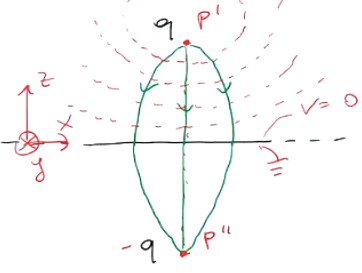
\includegraphics[width=0.5\linewidth]{metodo_immagini}
\caption{Metodo delle immagini}
\end{figure} 
La soluzione trovata come somma dei potenziali della carica reale e della carica immagine
è armonica e rispetta la condizione al contorno del problema di partenza $(V(z=0)=0)$ sarà
quindi soluzione del problema iniziale senza carica immagine.

\subparagraph{Linea bifilare in prossimità del terreno}
Utilizzando ancora il metodo delle immagini si può calcolare il campo generato da una linea
bifilare in prossimità del suolo.
\begin{figure}[h!]
\centering
 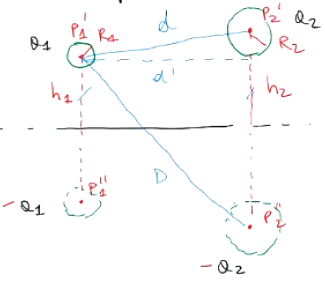
\includegraphics[width=0.5\linewidth]{linea_bifilare_terreno}
\caption{Metodo delle immagini su una linea bifilare}
\end{figure} 
Applicando il PSE
\begin{align*}
V_1 &= -\frac{\sigma_1 R_1 2\pi}{2\pi\varepsilon_0}\ln R_1 -
\frac{\sigma_2 R_2 2 \pi}{2 \pi \varepsilon_0}\ln d - 
\frac{\sigma_1 R_1 2 \pi}{2\pi \varepsilon_0} \ln(2 h_1) -
\frac{\sigma_2 R_2 2 \pi}{2\pi\varepsilon_0} \ln D \\
V_1 &= -\frac{Q_1}{2\pi\varepsilon_0} \ln(2 h_1 R_1) - 
\frac{Q_2}{2\pi\varepsilon_0} \ln (dD)\\
V_2 &= -\frac{Q_1}{2\pi\varepsilon_0} \ln(dD) - 
\frac{Q_2}{2\pi\varepsilon_0} (2h_2R_2)
\end{align*}
Nel caso di induzione completa si può calcolare la capacità
$$
C = \frac{\cancel{Q_1}}{\frac{\cancel{Q_1}}{2\pi\varepsilon_0}\left[-\ln(2h_1R_1)+\ln(dD)+\ln(dD)-\ln(2h_2R_2)\right]} = 
\frac{2\pi\varepsilon_0}{\ln\left[\frac{(dD)^2}{4h_1h_2R_1R_2}\right]}
$$
Applicando il teorema di Pitagora possiamo sostituire $D^2 = d^2 + (h_1+h_2)^2$
$$
C = \frac{2\pi\varepsilon_0}{\ln\left[\frac{d^2}{R_1R_2} 
\frac{\left[d^2+(h_1+h_2)^2\right]}{4h_1h_2} \right]}
$$
Se $h_1$ e $h_2$ tendono ad infinito, il coefficiente al 
denominatore che li contiene tende ad 1
$$
C \to \frac{2\pi\varepsilon_0}{\ln\left(\frac{d^2}{R_1R_2}\right)}
$$
Soluzione identica a quella trovata nel caso precedente in
assenza del terreno.

\subparagraph{Realizzazione di un induttore con un condensatore}
Sia dato un doppio bipolo con parametro $G$ conduttanza di
\textit{girazione}, le sue equazioni caratteristiche sono:
$$
\begin{cases}
i_1 = G v_2\\
i_2 = -G v_1
\end{cases}
$$
\begin{figure}[h!]
\centering
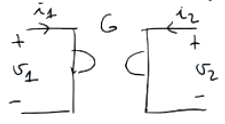
\includegraphics[width=0.3\linewidth]{giratore}
\caption{Giratore}
\end{figure}
Si realizza mediante dispositivi elettronici come 
amplificatori operazionali.

Connettendo ad una porta del giratore un condensatore la 
caratteristica diventa:
$$
\begin{aligned}
i_2 &= -C \frac{dv_2}{dt}\\
-Gv_1 &= -C\frac{d}{dt}\left(\frac{i_1}{G}\right)\\
v_1 &= \frac{C}{G^2}\frac{d}{dt}i_1 = L_{eq} \frac{d}{dt}i_1
\end{aligned}
$$
\begin{figure}[h!]
\centering
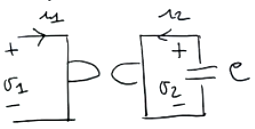
\includegraphics[width=0.3\linewidth]{giratore_con_condensatore}
\caption{Giratore con condensatore}
\end{figure}

\section{Materiali dielettrici}
E il loro modello elettromagnetico

\begin{itemize}
 \item Cariche ``legate'' nei dielettrici
 \item Cariche ``libere'' nei conduttori
\end{itemize}
Si usano queste due distinzioni macroscopiche anche se è possibile
assistere a spostamenti macroscopici di cariche anche nei dielettrici
durante le scariche disruptive e la rottura della relativa 
\textit{rigidità dielettrica}.

Quando il dielettrico è sottoposto ad un campo esterno, questo esercita 
una forza sulle cariche deformando la struttura del materiale e 
producendo così un campo differente, questo fenomeno prende il nome
di \textit{polarizzazione elettrica} e corrisponde ad un piccolo
spostamento delle cariche legate nel dielettrico a causa di un campo
esterno.
\subsection{Il dipolo elettrico}
Il dipolo elettrico è costituito da due cariche uguali e opposte
situate a distanza $d$. In queste condizioni, potenziale e campo 
dipendono dal \textit{momento di dipolo}.
$$
\vec{p} = qd \frac{(\vec{r}_{p'}-\vec{r}_{p''})}{|\vec{r}_{p'}-\vec{r}_{p''}|}
$$
\begin{figure}[h!]
\centering
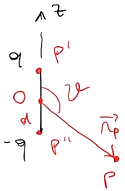
\includegraphics[width=0.2\linewidth]{dipolo_elettrico}
\caption{Dipolo elettrico}
\end{figure}

In questa configurazione è semplice calcolare il potenziale:
$$
V(P) = \frac{q}{4\pi\varepsilon_0}\left[ \frac{1}{|\vec{r}_p-\vec{r}_{p'}|} - \frac{1}{|\vec{r}_p-\vec{r}_{p''}|} \right] = 
\frac{q}{4\pi\varepsilon_0} \left[ \frac{|\vec{r}_p-\vec{r}_{p''}|-|\vec{r}_p-\vec{r}_{p'}|}
{|\vec{r}_p-\vec{r}_{p'}|\cdot|\vec{r}_p-\vec{r}_{p''}|} \right]
$$
Allontanandosi dal dipolo $|\vec{r}_p| \gg |\vec{r}_{p'}|,|\vec{r}_{p''}|$ quindi il potenziale
diventa:
$$
V(P) = \frac{q}{4\pi\varepsilon_0} \left[ \frac{|\vec{r}_p-\frac{d}{2}\vec{e}_z|-|\vec{r}_p + \frac{d}{2}\vec{e}_z|}
{|\vec{r}_p-\vec{r}_{p'}|\cdot|\vec{r}_p-\vec{r}_{p''}|} \right] = 
\frac{q}{4\pi\varepsilon_0} \left[ \frac{\sqrt{r_p^2 + \left(\frac{d}{2}\right)^2-r_p d \cos \vartheta} - \sqrt{r_p^2 + \left(\frac{d}{2}\right)^2 + r_p d \cos \vartheta}}
{|\vec{r}_p-\vec{r}_{p'}|\cdot|\vec{r}_p-\vec{r}_{p''}|} \right] 
$$
Sviluppando in serie il numeratore si ottiene
$$
 \sqrt{1 + \left(\frac{d}{2r_p}\right)^2- 
\frac{d}{r_p} \cos \vartheta} - \sqrt{1 + \left(\frac{d}{2r_p}\right)^2 + \frac{d}{r_p} \cos \vartheta} \simeq %rigo 2
\left(1 + \frac{d}{2r_p} \cos \vartheta\right) - \left(1 - \frac{d}{2r_p} \cos \vartheta\right)
\simeq d\cos\vartheta
$$

In conclusione il potenziale in un punto lontano dal dipolo sarà
$$
V(P) \simeq \frac{q}{4\pi\varepsilon_0} \frac{d\cos\vartheta}{r_p^2} = \frac{1}{4\pi\varepsilon_0}
\frac{\vec{p}\cdot\vec{r}_p}{r_p^3}
$$
$$
\vec{E}(P) = -\nabla V = \frac{3\left(\vec{p}\cdot\vec{r}_p\right)\vec{r}_p - r_p^2\vec{p}}{4\pi\varepsilon_0r_p^5}
$$
Si osserva quindi che la funzione potenziale decresce come $\frac{1}{r_p^2}$ mentre il 
campo decresce come $\frac{1}{r_p^3}$

\subparagraph{Dipolo in un campo elettrico esterno}
\begin{figure}[h!]
\centering
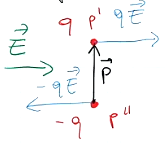
\includegraphics[width=0.2\linewidth]{dipolo_nel_campo}
\caption{Dipolo immerso in un campo elettrico $\vec{E}$}
\end{figure}
Supponiamo di avere un dipolo di momento $\vec{p}$ e applichiamo un campo esterno $\vec{E}$,
questo eserciterà una forza sulla carica $q$ ed una opposta sulla carica $-q$, la risultante delle 
due forze sarà nulla ma producono una coppia sul bipolo esprimibile come
$$
\left(\vec{r}_{p'} - \vec{r}_{p''}\right)\times q\vec{E} = \vec{p}\times\vec{E}
$$
La coppia tende a far ruotare il bipolo elettrico e l'interazione ammette due condizioni di 
equilibrio determinate da $\vec{p}\times\vec{E} = 0 $

Stabile se il dipolo è allineato con il campo, instabile se è allineato ma in verso opposto,
una piccola perturbazione lo farebbe ruotare di 180\textdegree

Questa caratteristica permette di discernere le sostanze in due categorie: apolari ($O_2$) e polari
($H_2O$) se queste presentano o meno momenti di dipolo permanenti.

Esistono vari tipi di polarizzazione: per \textit{deformazione} se una sostanza apolare, sotto 
l'azione di un campo elettrico, subisce lo spostamento delle cariche legate producendo 
un momento di dipolo.
Oppure per \textit{orientamento} che riguarda le sostanze polari che a temperatura ambiente
presentano un momento di dipolo medio nullo, pur essendo le singole molecole (o atomi) polari.
L'agitazione termica determina l'orientamento casuale dei dipoli elementari.

\begin{figure}[h!]
 \centering
 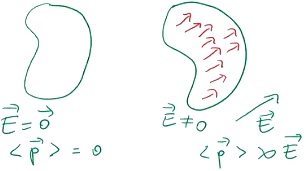
\includegraphics[width=0.4\linewidth]{polarizzazione_deformazione}
 \caption{Polarizzazione per deformazione}
\end{figure}


\begin{figure}[h!]
 \begin{subfigure}{.5\textwidth}
 \centering
 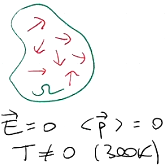
\includegraphics[width=0.45\linewidth]{sost_apolare_a_media_nulla}
 \caption{Sostanza apolare}
 \end{subfigure} 
 \begin{subfigure}{.5\textwidth}
\centering
 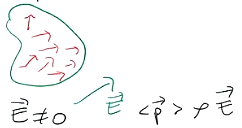
\includegraphics[width=0.8\linewidth]{sost_apolare_polarizzata}
 \caption{Sostanza polarizzata}
 \end{subfigure}
 \caption{Polarizzazione per orientamento}
\end{figure}

Dal punto di vista fisico i due fenomeni sono diversi ma dal punto di vista modellistico
entrambi hanno un momento di dipolo allineato con il campo esterno.
Si introduce quindi nel volume elementare $\Delta\Omega$ il momento di dipolo medio
$$
<\vec{p}> = \vec{P}(Q,t)\cdot \text{Vol}(\Delta\Omega)
$$
dove $\vec{P}(Q,t)$ è il vettore (intensità di) di polarizzazione elettrica ed ha il significato 
di una densità di momento di dipolo media
$$
<\vec{p}> = \frac{N<\vec{p}_a>}{\text{Vol}(\Delta\Omega)}\cdot \text{Vol}(\Delta\Omega)
$$
Per descrivere le cariche legate all'interno del volumetto può essere comodo immaginare la materia
costituita da tanti dipolini elementari.
